\section{Simplifying NTK into atomic units: Roles of gates, weights, width and depth}

\subsection{Neural Path Kernel: Composition of Base Kernels}
\begin{definition}
Define the NPK matrix to be  $H_{\Theta}\eqdef\Phi^\top_{\Theta}\Phi_{\Theta}$, where $\Phi_{\Theta}=(\phi_{x_1,\Theta},\ldots,\phi_{x_n,\Theta})\in\R^{P\times n}$ is the NPF matrix.
\end{definition}
\begin{comment}
As a result, it turns out that, depending on the network architecture, the NPK has interesting structure/form. In FC-DNN, the NPK involves product of base kernels (\Cref{def:layerkernel},\Cref{lm:productkernel}) corresponding to the binary gating features of the various layers. In ResNet with $b$ skip connections there are $2^b$ sub-FC-DNNs and the NPK is a sum of the NPKs of these sub-FC-DNNs (\Cref{lm:sumofproduct}). Further, in CNNs due to weight sharing, the NPK has a rotationally invariant form (\Cref{lm:cnnnpk}). In what follows, we define the NPK matrix to be  $H_{\Theta}\eqdef\Phi^\top_{\Theta}\Phi_{\Theta}$, where $\Phi_{\Theta}=(\phi_{x_1,\Theta},\ldots,\phi_{x_n,\Theta})\in\R^{P\times n}$ is the NPF matrix.
\end{comment}
\begin{definition}\label{def:cnnlambda}
 Define $\Lambda_{\Theta}(i,x,x_{s'}) \eqdef \left|\{p\in[P]\colon  \I_0(p)=i, A_{\Theta}(x_s,p)= A_{\Theta}(x_{s'},p)=1\}\right|$ to be total number of `active' paths for both $x_s$ and $x_{s'}$ that pass through input node $i$.
\end{definition}
%\subsection{NPK of FC-DNN: Product Kernel }
%\input{cnpkexample}
%\subsection{Neural Path Kernel : Similarity based on active sub-networks}
\begin{definition}[Layer-wise Kernel]\label{def:layerkernel} Let $G_{x,\Theta}(\cdot,l)\in\R^w$ be $w$-dimensional feature of the gating values in layer $l$ for input $x\in\R^{\din}$.  Define layer-wise kernels:
\begin{align*}
H^{\text{lyr}}_{l,\Theta}(s,s')\eqdef\ip{G_{x_s,\Theta}(\cdot,l)G_{x_{s'},\Theta}(\cdot,l)}
\end{align*}
\end{definition}
\begin{lemma}[Product Kernel]\label{lm:productkernel}
 Let $H^{\text{fc}}$ denote the NPK of a FC-DNN, and for $D\in\R^{\din\times\din}$ be a diagonal matrix with strictly positive entries, and $u,u'\in\R^{\din}$ let $\ip{u,u'}_{D}=\sum_{i=1}^{\din}D(i)u(i)u'(i)$.
\begin{align*}
H^{\text{fc}}_{\Theta}(s,s')= \ip{x_s,x_{s'}}_{\Lambda(\cdot,x_s,x_{s'})}=\ip{x_s,x_s'}\Pi_{l=1}^{d-1}H^{\text{lyr}}_{l,\Theta}(s,s')\end{align*}
\end{lemma}


\subsection{Main Theorem: $\text{NTK}^{\text{fixed-gate}}\propto\text{NPK}$}
\begin{assumption}\label{assmp:main}
(i) $\Tv_0$ is statistically independent of $\Tf_0$ (ii) $\Tv_0$ are i.i.d symmetric Bernoulli over $\{-{\sigma},+{\sigma}\}$. 
\end{assumption}

\begin{theorem}\label{th:main} Let $\sigma=\frac{\sigfc}{\sqrt{w}}$ in \Cref{assmp:main}. As $w\ra\infty$, for FC-DGN we have: 

\begin{align*}
\kv_{\Tdgn_0}(x,x')&\stackrel{(a)}\ra d \sigma^{2(d-1)} H_{\Tf_0}(x,x')\\ 
%&\stackrel{(a)}{=} d \sigfc^{2(d-1)}\langle x,x'\rangle\cdot \Pi_{l=1}^{d-1} \left(\frac{\langle G_{x,\Tf_0}(l), G_{x',\Tf_0}(l) \rangle}{w}   \right)\\
%&\stackrel{(a)}\propto \langle x,x'\rangle\cdot \Pi_{l=1}^{d-1} \left(\frac{\langle G_{x,\Tf_0}(l), G_{x',\Tf_0}(l) \rangle}{w}   \right)\\
&\stackrel{(b)}= \langle x,x'\rangle\cdot \Pi_{l=1}^{d-1} \frac{H^{\text{lyr}}_{l,\Tf_0}(x,x')}{w}
\end{align*}

\end{theorem}
\subsection{Pictorial Illustration}
\FloatBarrier
\begin{figure}[h]
\centering
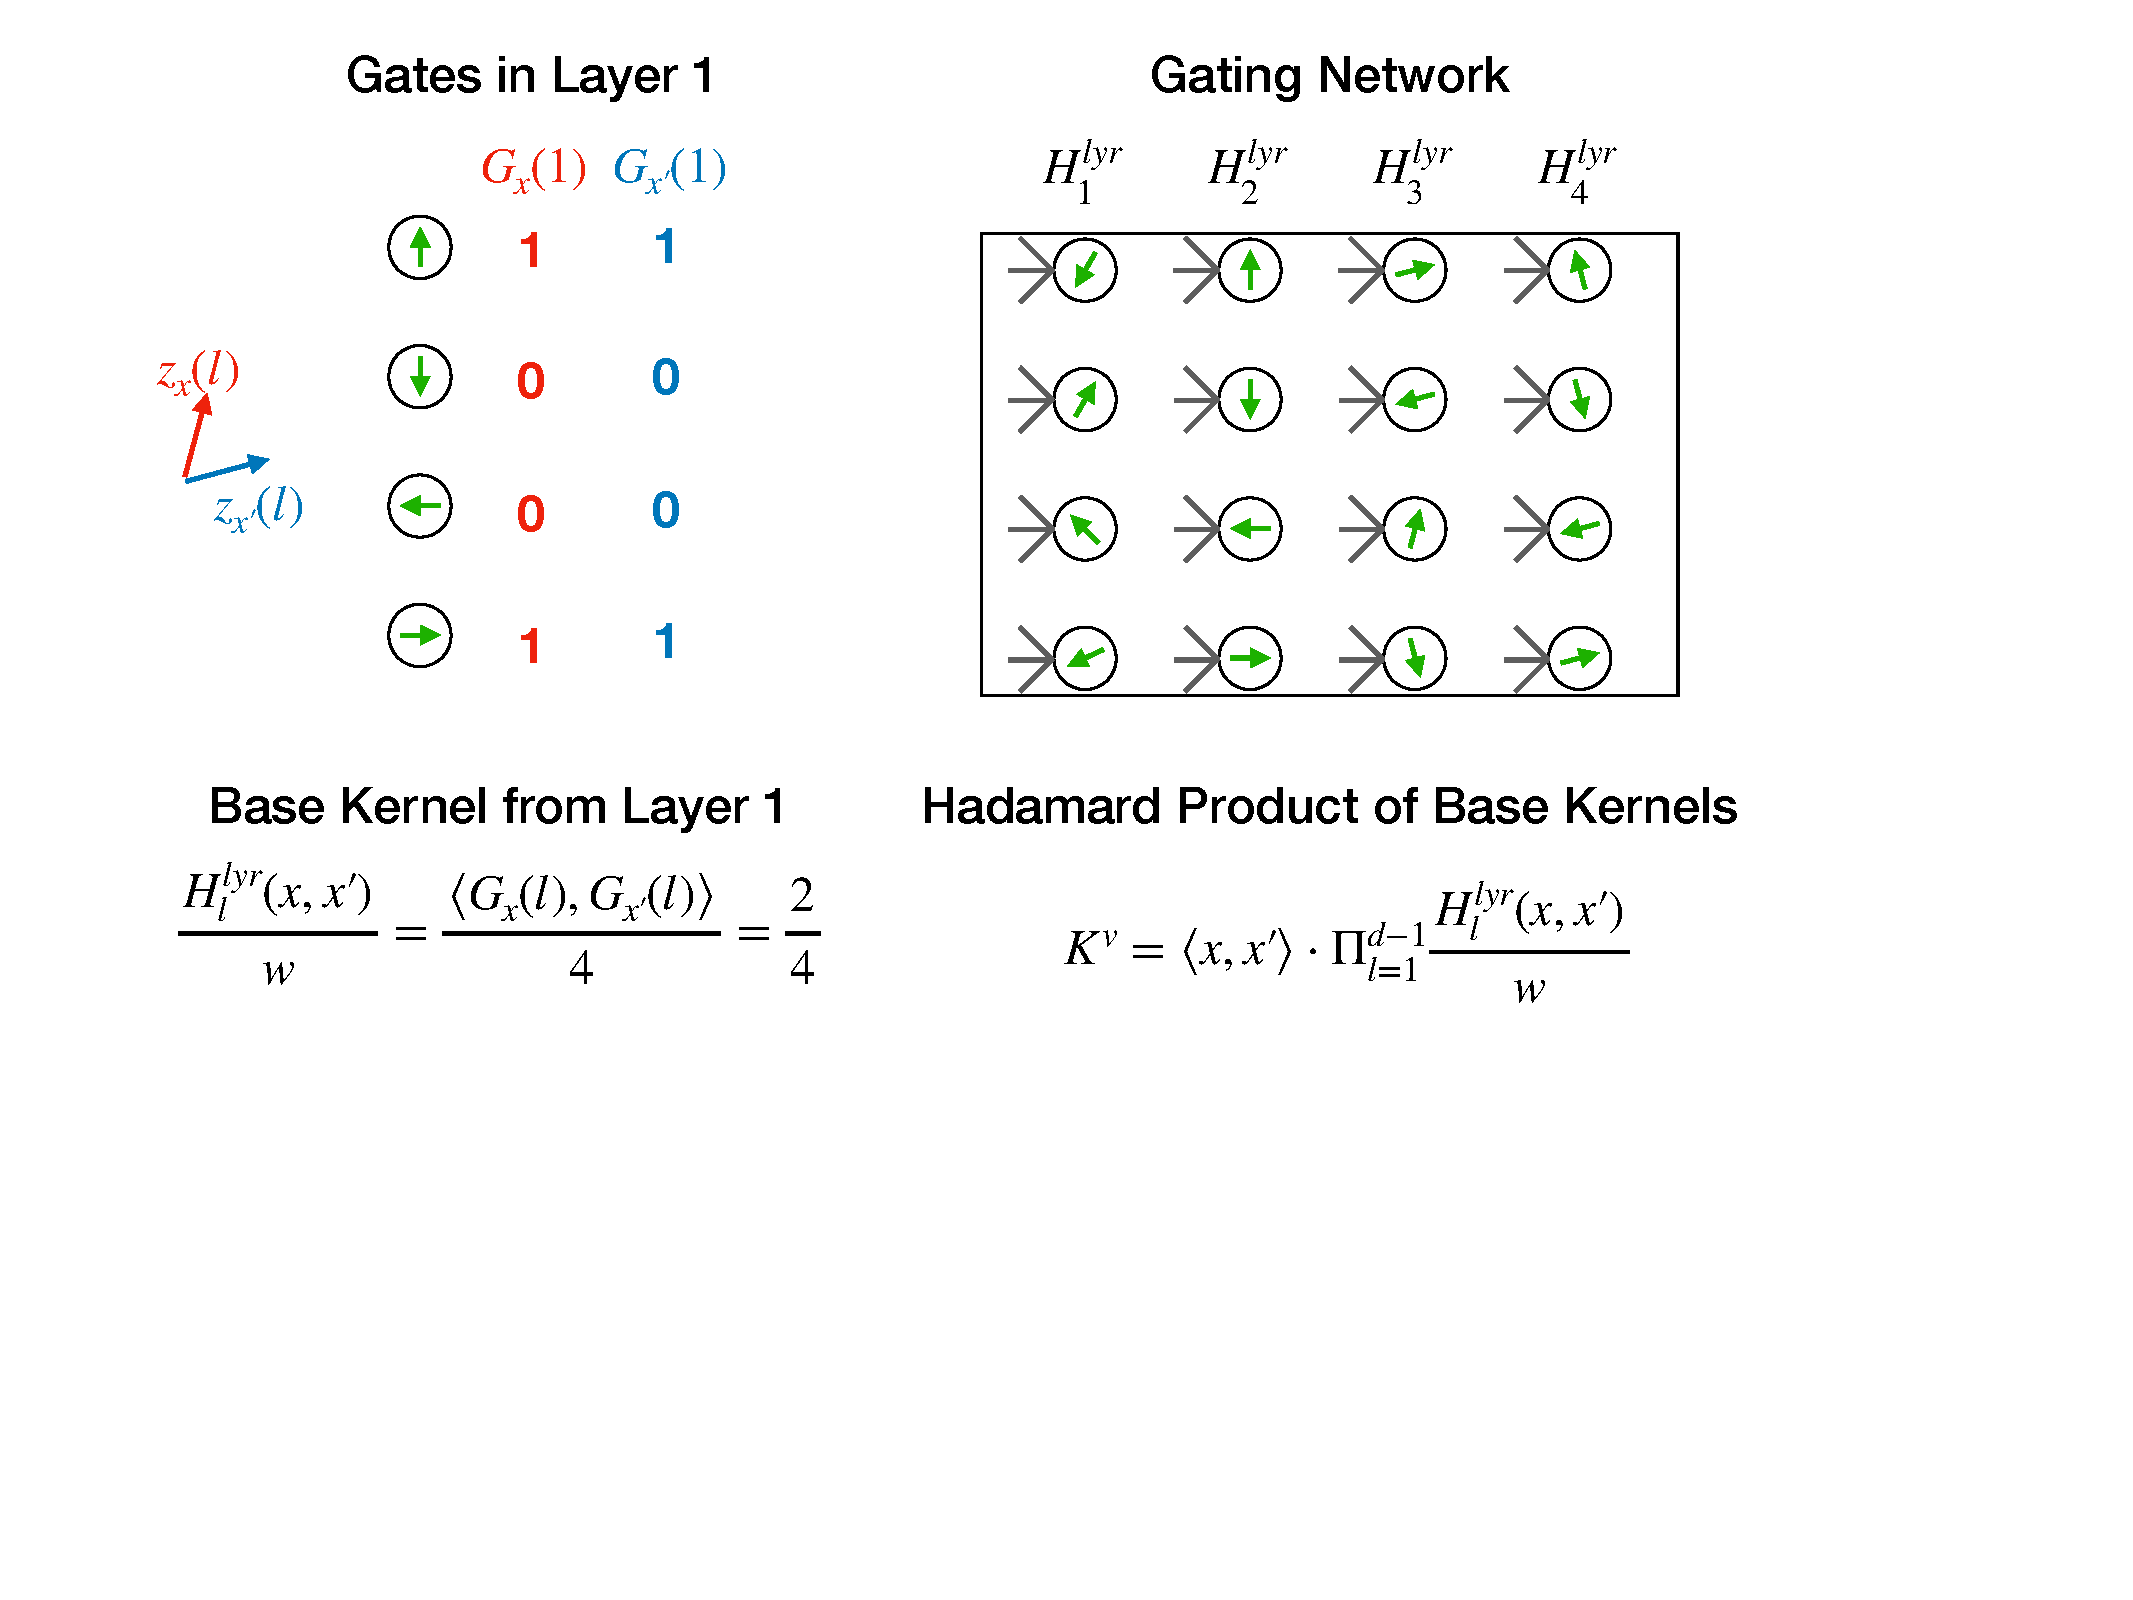
\includegraphics[scale=0.25]{figs/overall.pdf}
\end{figure}